\section{User Interface}
The user interface consists of a main view and a view where users can edit their Feedback.
\subsection{Main View}
The app is controlled with a main view that allows selecting from three sub-views with specific functionality. A view to send Feedback (Figure \ref{fig_send}), a map view (Figure \ref{fig_map}) and a profile view which lists the user's feedback (Figure \ref{fig_profile}). This is done via interactive buttons and controls familiar to most smartphone users.\\

\begin{figure}[H]
\minipage{0.32\textwidth}
  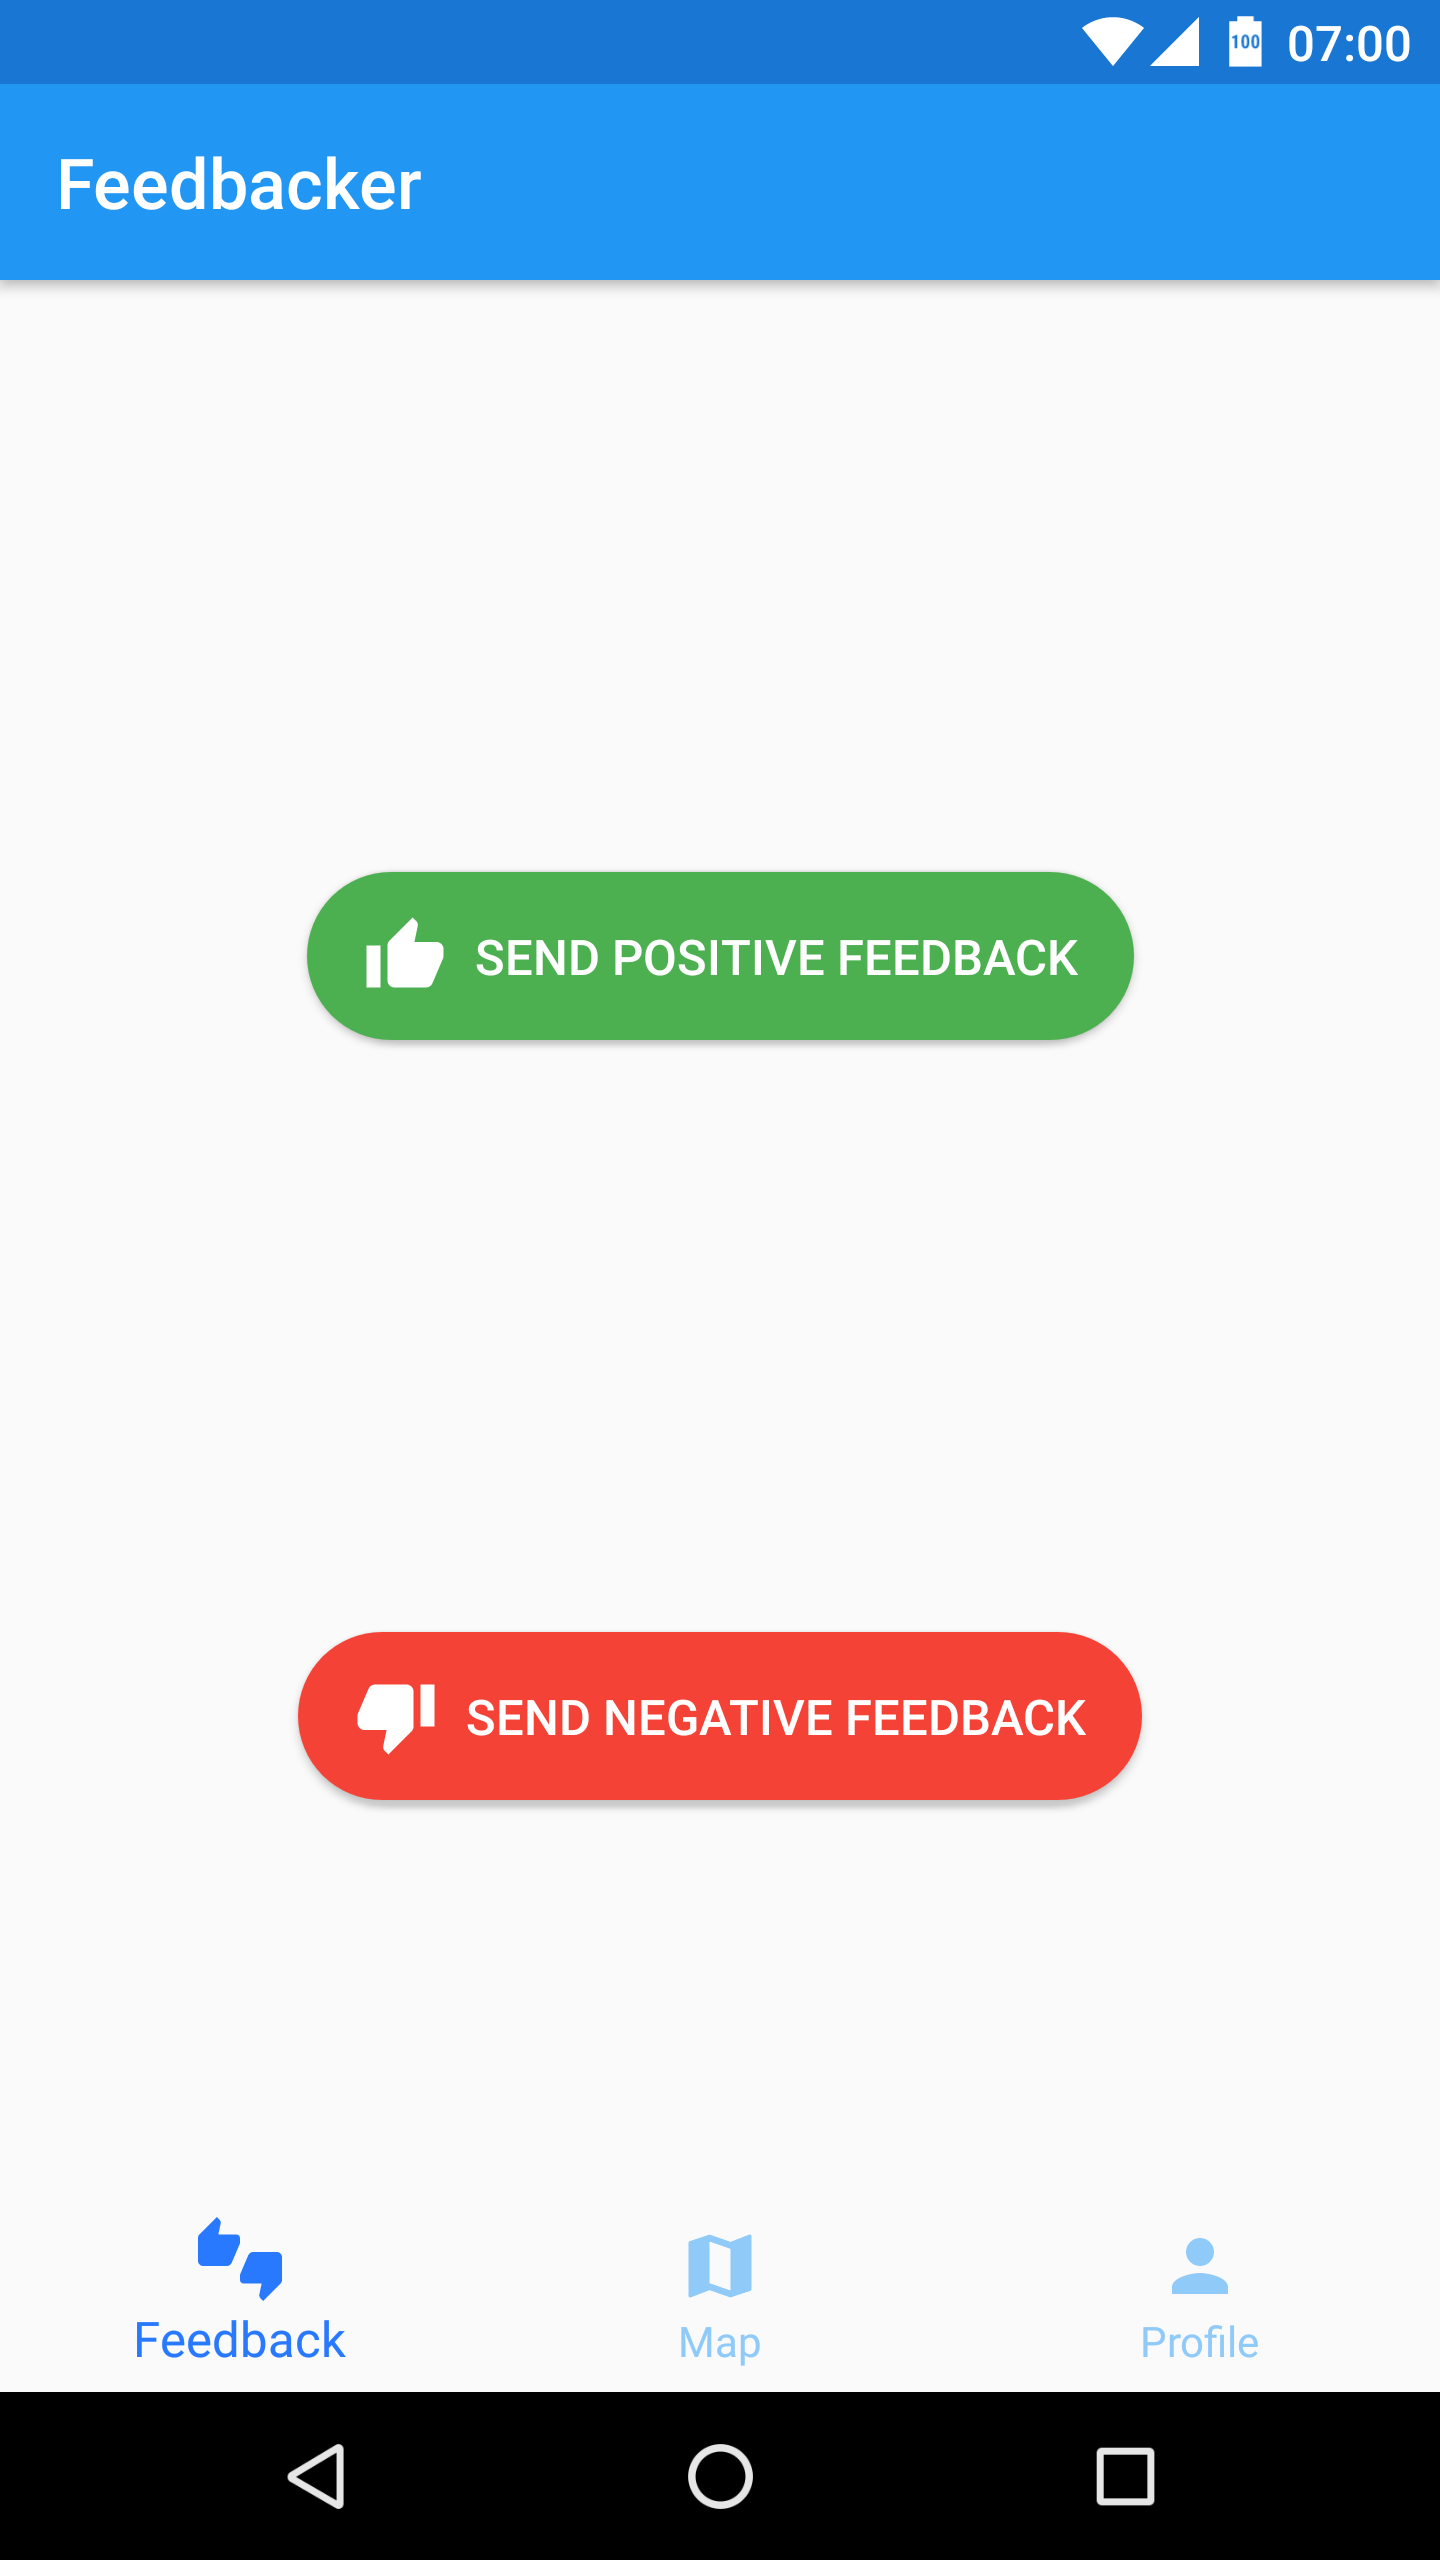
\includegraphics[width=\linewidth]{bilder/Screenshot_Send_Feedback.png}
  \caption{Feedback View Android}\label{fig_send}
\endminipage\hfill
\minipage{0.32\textwidth}
  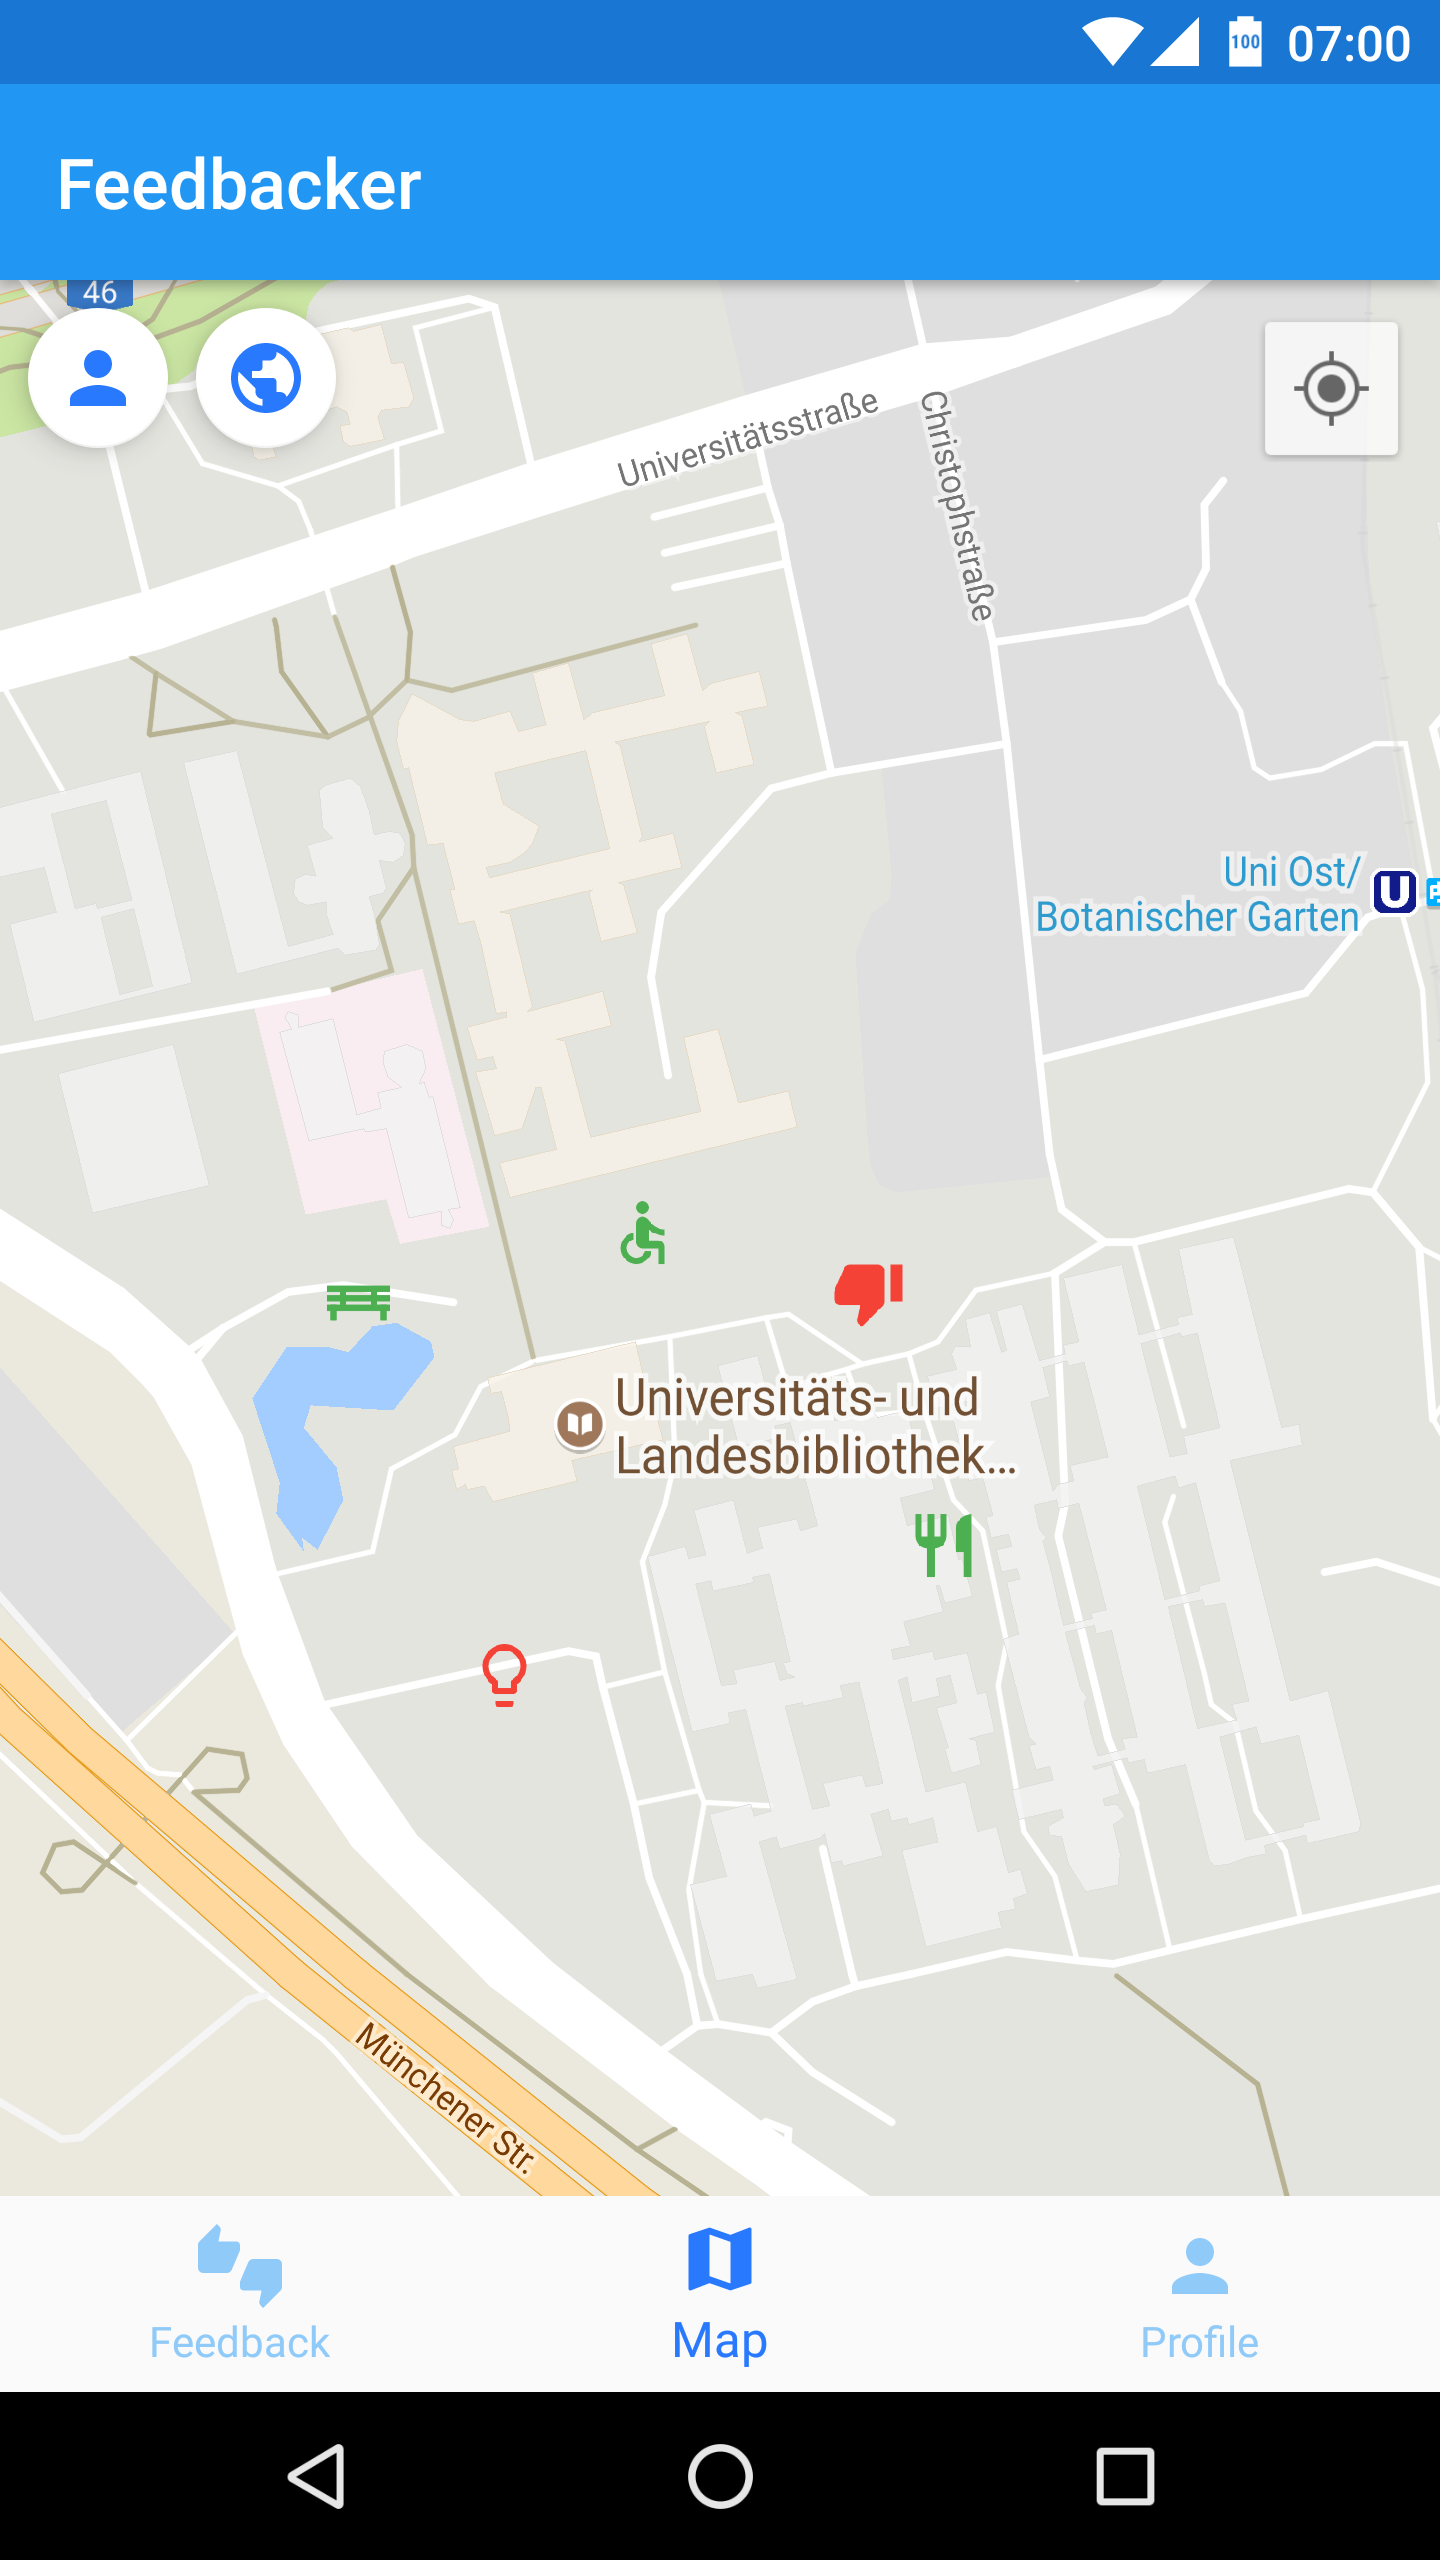
\includegraphics[width=\linewidth]{bilder/Screenshot_Map.png}
  \caption{Map View Android}\label{fig_map}
\endminipage\hfill
\minipage{0.32\textwidth}%
  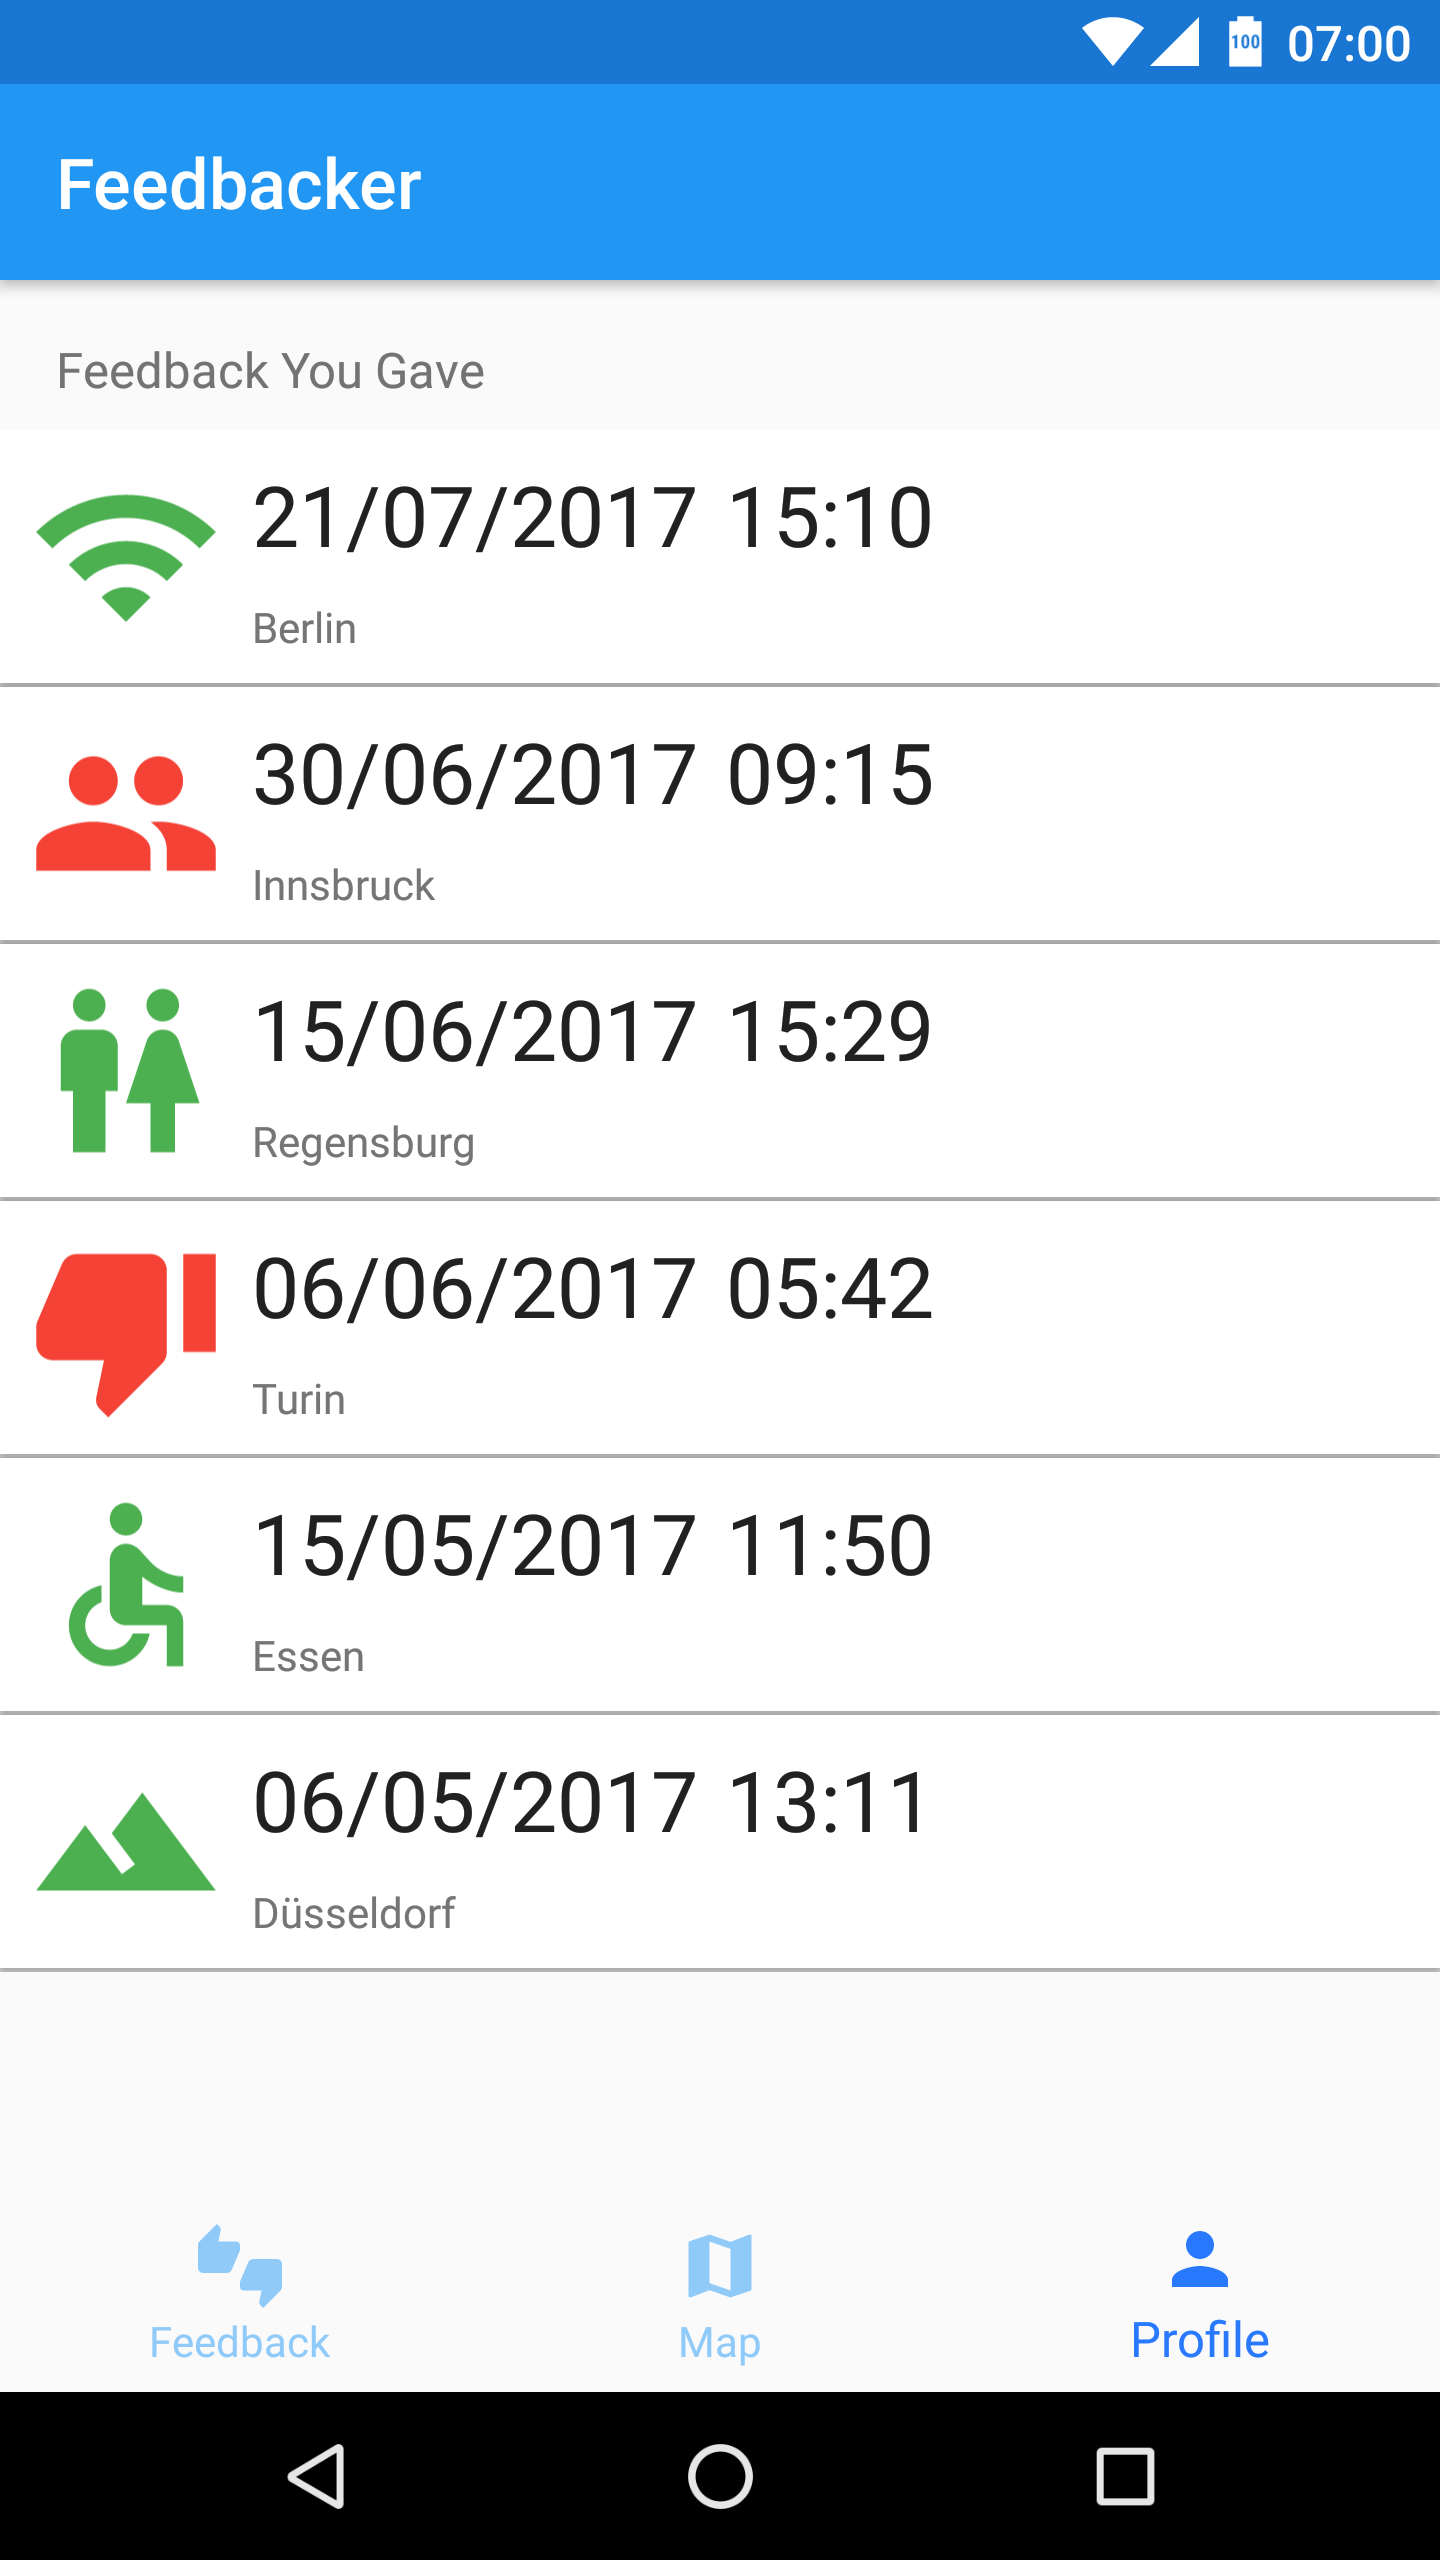
\includegraphics[width=\linewidth]{bilder/Screenshot_Profile.png}
  \caption{Profile View Android}\label{fig_profile}
\endminipage
\end{figure}

\subsubsection{Feedback View} \label{ssec:send}
This only displays two button to send positive and negative feedback, respectively. Clicking on either of these buttons will send a feedback of that type.


\subsubsection{Map View} \label{ssec:map}
This view displays a map with markers at the locations where feedback has been sent. Clicking on a Marker will open a popup with time and date of the feedback as well as the descriptive text if the feedback's sender provided one. Feedbacks provided by the user itself have a button to edit this feedback. \newline
In the top left corner there are buttons that allow the user to choose whether personal feedbacks and public feedbacks provided by other users should be displayed on the map.


\subsubsection{Profile View} \label{ssec:profile}
This view shows a list of the feedbacks provided by the user. Each feedback item has an icon based on the feedback's category as well as the time, date and city of that specific feedback.


\subsection{Feedback Edit View}
This view gives the user the ability to edit a feedback. This view can be reached via three ways. By sending a new feedback, via a marker on the map and from the list in the profile view. \newline

\begin{figure}[H]
  \begin{center}
    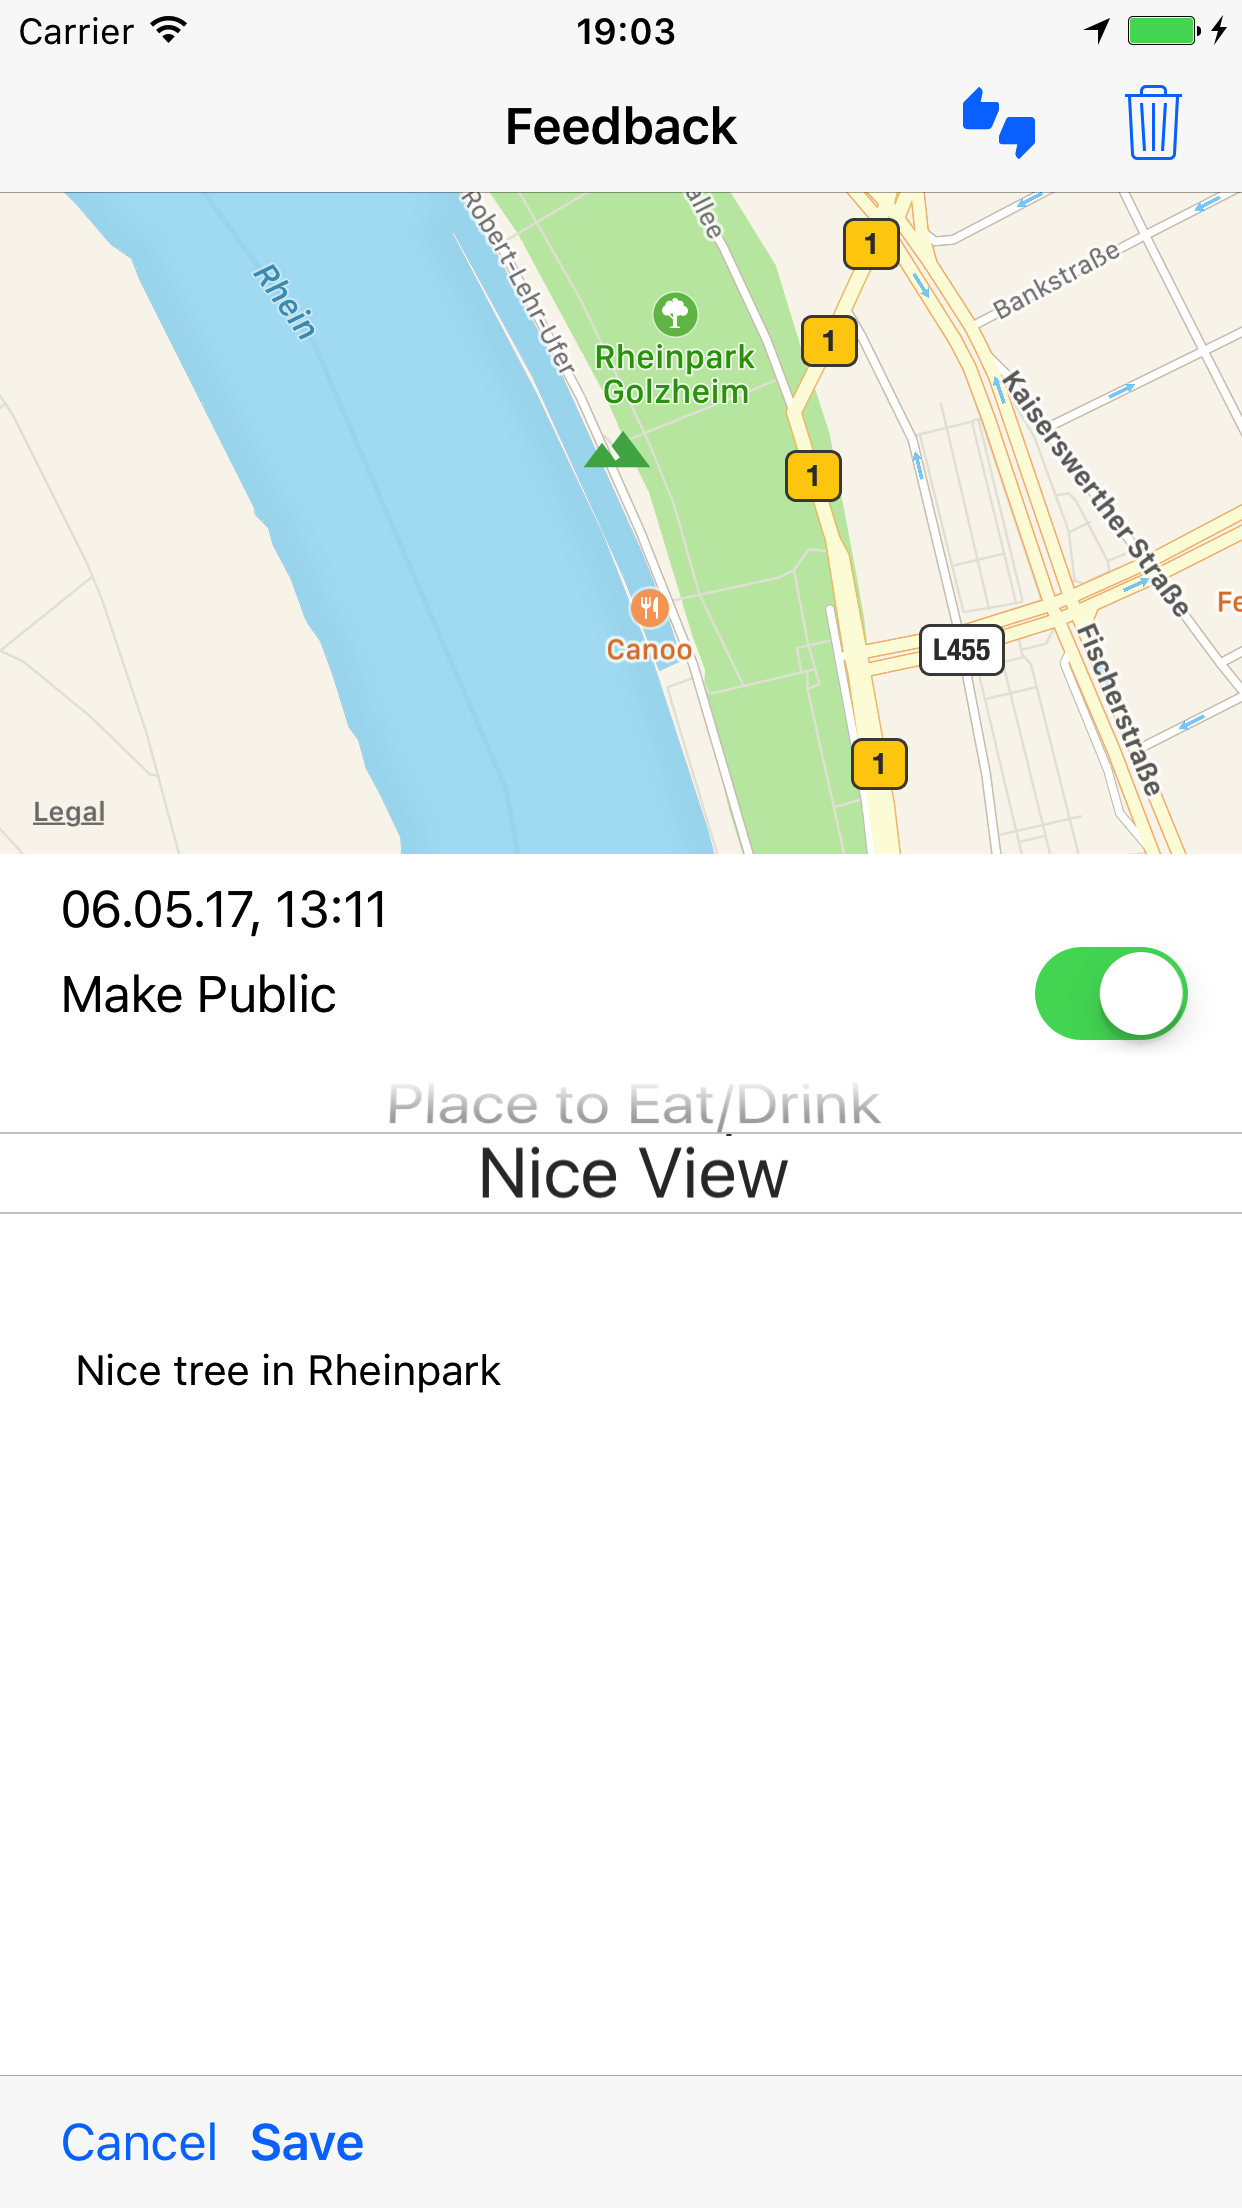
\includegraphics[width=0.32\textwidth]{bilder/Screenshot_Edit}
    \caption{Feedback Edit View iOS}\label{fig_edit}
  \end{center}
\end{figure}

\paragraph{View Components}
At the top of the layout there is a map marking the location of the feedback to give the user an orientation where his feedback is placed on the map. Directly below the date and time at which the feedback has been sent is shown. These features are common to all types of feedbacks, as they are send directly when the user hits one of the send feedback buttons. \newline
A switch can be used to mark the feedback as public, which will display that feedback for other users on the map. By default the switch is off. \newline
The category can be chosen from a menu. Depending on the kind of feedback (positive/negative), the menu will show the corresponding options listed in Table \ref{table:categories} on page \pageref{table:categories}. At the bottom of the layout there is a textbox for the user to provide a descriptive text for the feedback.

\paragraph{Toolbar Actions}
At the upper toolbar the user can switch the kind of the feedback as well as delete the feedback. Both of these actions will show a popup to confirm this action as they delete the currently selected category or the whole feedback, respectively. \newline
At the bottom there is a save and a cancel button. The save button will save all the edits the user has made to his feedback and the cancel button will discard all edits.
